% vim: set tw=78 sts=2 sw=2 ts=8 aw et ai:
TODO

\begin{figure}
  \centering
  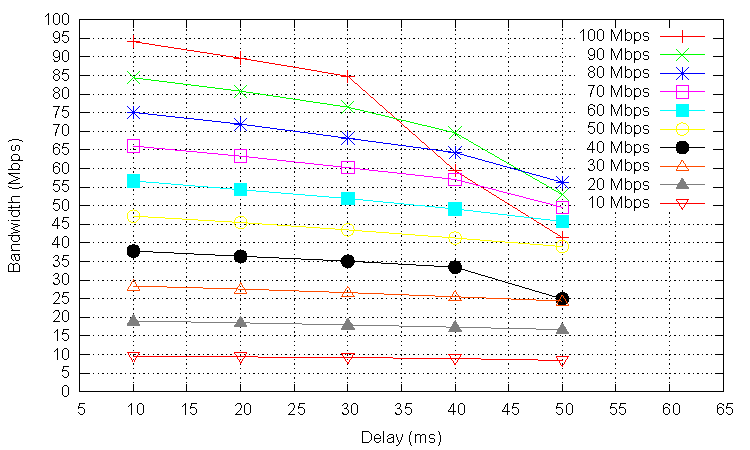
\includegraphics[width=\textwidth]{img/test-udp}
  \caption{Single UDP tunnel throughput}
  \label{fig:udp}
\end{figure}

\begin{figure}
  \centering
  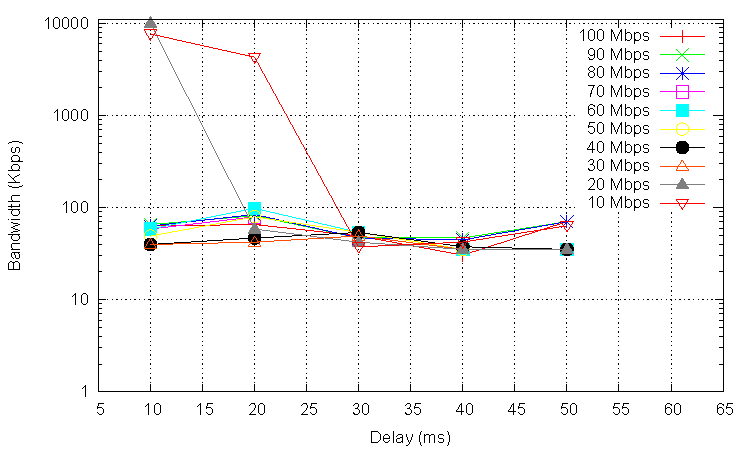
\includegraphics[width=\textwidth]{img/test-tcp}
  \caption{Single TCP tunnel throughput}
  \label{fig:tcp}
\end{figure}

\begin{figure}
  \centering
  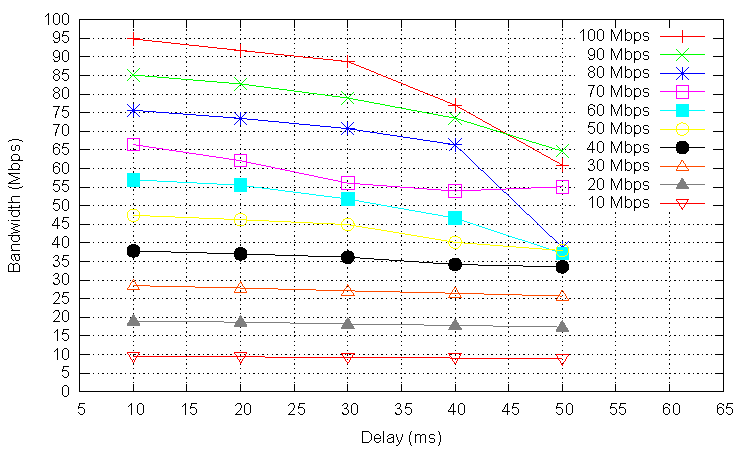
\includegraphics[width=\textwidth]{img/test-mptcp}
  \caption{UDP and TCP tunnels throughput}
  \label{fig:mptcp}
\end{figure}

\begin{figure}
  \centering
  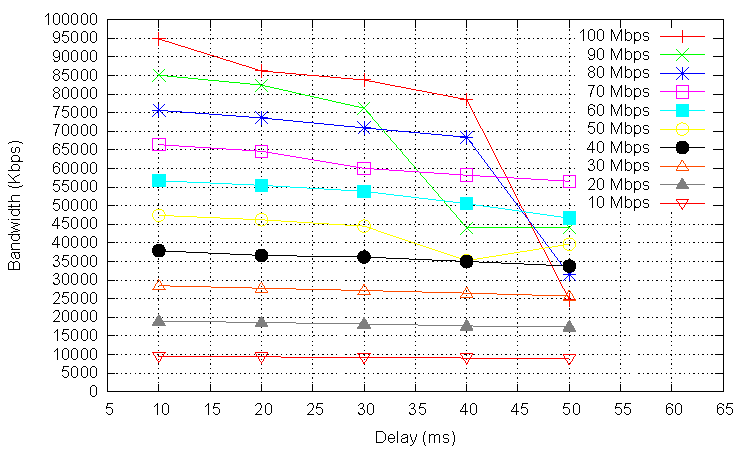
\includegraphics[width=\textwidth]{img/test-mptcp-05}
  \caption{UDP and TCP tunnels throughput, half buffer size}
  \label{fig:mptcp-0.5}
\end{figure}

\begin{figure}
  \centering
  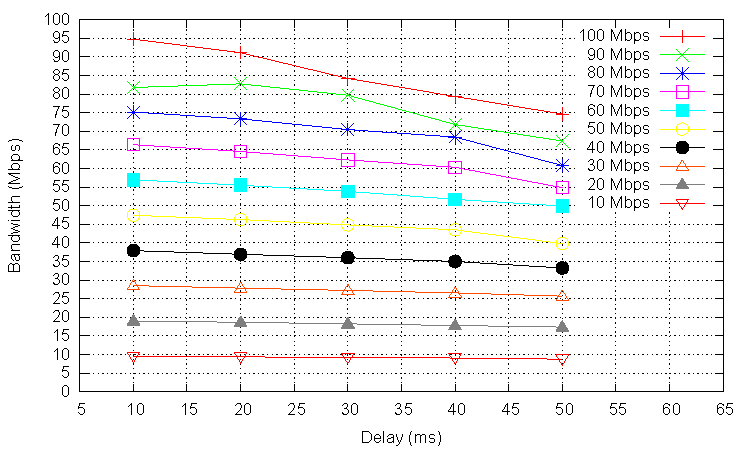
\includegraphics[width=\textwidth]{img/test-mptcp-2}
  \caption{UDP and TCP tunnels throughput, double buffer size}
  \label{fig:mptcp-2}
\end{figure}

\begin{figure}
  \centering
  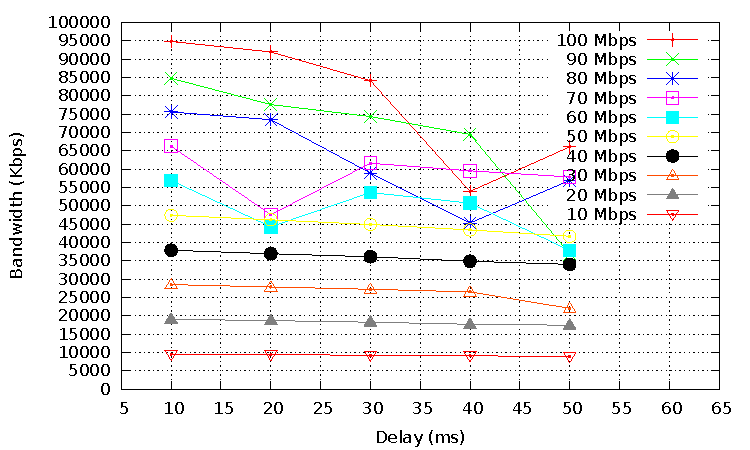
\includegraphics[width=\textwidth]{img/test-mptcp-4}
  \caption{UDP and TCP tunnels throughput, 4 times buffer size}
  \label{fig:mptcp-4}
\end{figure}

